\documentclass[titlepage,a4paper]{jsarticle}
\usepackage{../sty/import}% 各種パッケージインポート
\usepackage{../sty/title}% タイトルページの変更

%% タイトルページの変数
% レポートタイトル
\title{環境経済学期末試験}
% 提出日
\expdate{\today}
% 科目名
\subject{環境経済学}
% 分野
\class{情報経営システム工学分野}
% 学年
\grade{B3}
% 学籍番号
\mynumber{24336488}
% 記述者
\author{本間三暉}
% グループ名 % もし班があるやつならtitle_team.styを入れる
% \team{10}
% 共同実験者 % もし共同実験者が必要なやつならtitle_kyoudou.styを入れる
% \coauthor{%
% \textbf{学籍番号:} & \textbf{氏名:} \ \
% \textbf{学籍番号:} & \textbf{氏名:}\ \
% \textbf{学籍番号:} & \textbf{氏名:}\ \
% \textbf{学籍番号:} & \textbf{氏名:}\ \
% }
%
% 記載例:
%\coauthor{%
% 学籍番号:24567321 & 氏名:吉田 富美男 \
% 学籍番号:12345678 & 氏名:安藤 雅洋 \
% 学籍番号:13579234 & 氏名:雲居 玄道 \
%%

\begin{document}
% titleページ作成
\maketitle
\section{記述問題}
\subsection*{国際交渉の結果、ある国が二酸化炭素排出量をXトン削減する義務を負うことになった。
  そこで、 図\ref{環境図}のとおり、政府は、Raの限界削減コスト曲線を持つ企業Aに、Xaトンの削減量を、Rbの限界削減 コスト曲線を持つ企業Bに、Xbトンの削減量を割り当てたとする。
  ただし、X=Xa+Xbと仮定する。}
\begin{figure}[H]
  \centering
  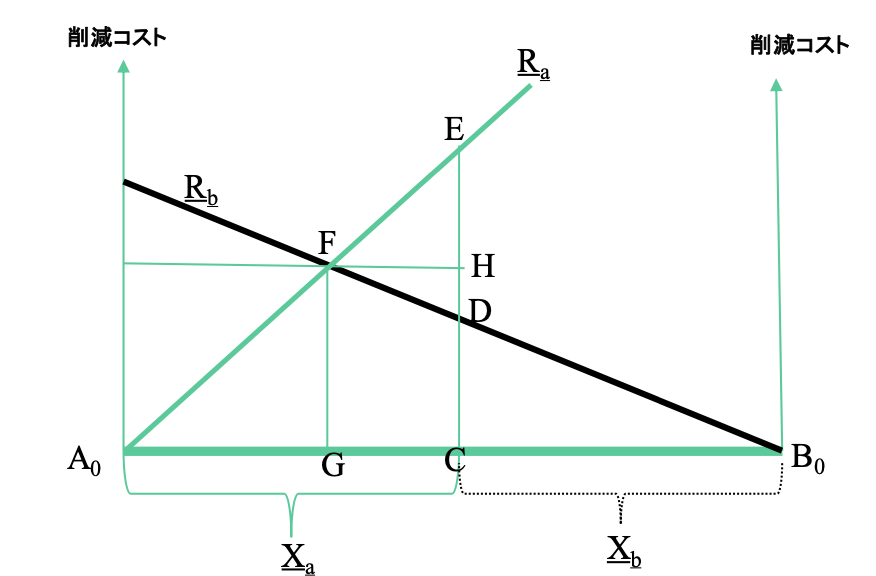
\includegraphics[width=12cm]{img/env.png}
  \caption{aa}
  \label{環境図}
\end{figure}

\subsection{二酸化炭素削減量取引を許さない場合の削減コストを求めよ。}
\subsection{二酸化炭素削減量取引を許す場合の削減コストを求めよ。}
\subsection{二酸化炭素削減量取引を許す場合と許さない場合の削減コストを比較せよ。}
\subsection{二酸化炭素削減量取引を許す場合の、取引量、取引価格を求めよ。}

\section{レポート課題}
\subsection*{道路輸送部門の脱炭素化を実現するために、自動車の電動化が必要不可欠である。
  自動車電動化の推進にどのような対策が必要か、ZEV(Zero Emission Vehicle)目標規制・クレジット取引制度をどう位置づけるか 等について、検討せよ。}
% 参考文献
\begin{thebibliography}{99}
  \bibitem{}
\end{thebibliography}

\end{document}
